\chapter{About web sessions}

When a user visits a website, it is often needed for the web application to remember which user it is interacting with. For this reason, the concept of a `web session' was invented. In this chapter we will see how web sessions work, and how their security can be improved.

\section{How web sessions work}\label{session-management}

To understand the need for web sessions, we first have to look at how web browsers communicate with web servers. The browser requests web pages by issuing \gls{http} requests to a web server \cite{Kurose2008}. The server subsequently responds to every request with an HTTP response containing the requested page. Unfortunately, HTTP is a stateless protocol, which means that the web server has no way of knowing whether two different requests come from the same user. Because of this, a mechanism is needed on top of HTTP to enable stateful communication between a web server and a client. This mechanism is known as a web session.

Web sessions work as follows:
\begin{enumerate}
	\item When the web server receives its first HTTP request from a particular client, it creates a \emph{session identifier} (also called a \gls{session id} or \gls{sid}) that it associates with this client. It then sends the newly generated SID to the client as part of the HTTP response.
	\item In subsequent communications, the client attaches the SID it received to every HTTP request it issues to the server. Because the web server has associated this SID with a particular client, it will know who it is interacting with.
\end{enumerate}

There are three ways in which session identifiers can be attached to requests and responses \cite{Jovanovic2006}. The first one, which is most common, makes use of \glspl{cookie} \cite{Kristol2001, Park2000}. Cookies are strings consisting of multiple name-value pairs which are set by the web server using the \texttt{Set-Cookie} HTTP header. Upon receiving a cookie, the browser stores it for a specified amount of time. It then attaches this cookie to every subsequent request made to the server\footnote{The actual access control policy is a bit more complicated and will be discussed in section \ref{access-control}.} that set the cookie by using HTTP's \texttt{Cookie} header. This process is graphically depicted in Figure \ref{fig:sessions-cookies}. It is clear that cookies are a very convenient mechanism for managing session identifiers. Because cookies can also be used for other purposes than session management, we will make a distinction between \emph{cookies} (which can be used for all sorts of state information) and \emph{\glspl{session cookie}} (which are cookies that store a SID) in this text.

\begin{figure}[ht]
	\centering
	\subfloat[via cookies]{
		\label{fig:sessions-cookies}
		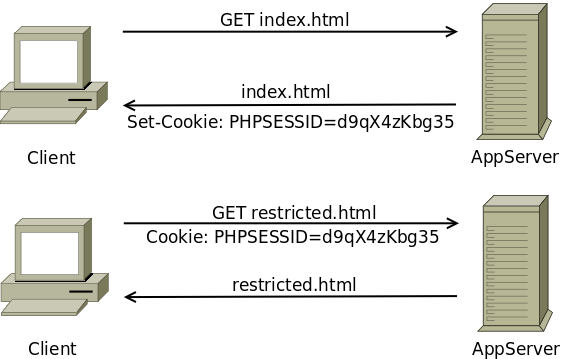
\includegraphics[width=.47\textwidth]{img/Sessions.png}
	}
	\subfloat[via URL rewriting]{
		\label{fig:url-rewriting}
		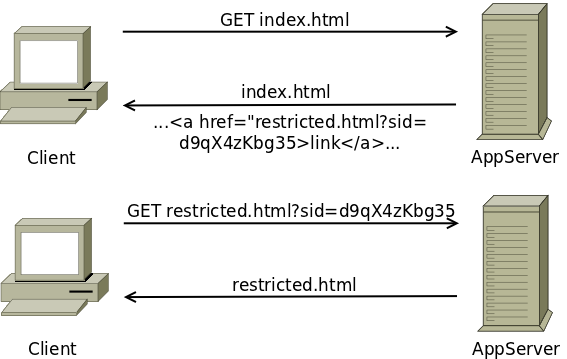
\includegraphics[width=0.47\textwidth]{img/url-rewriting.png}
	}
	\caption{Session management}
\end{figure}

The second possibility to include session information is via \emph{\gls{url} rewriting}. In this case, the web server appends the session ID as a parameter to every served URL that points to a page on the same server. Thus, when the user clicks a link on the served page, the request that is made contains the session ID as a parameter, and the server will know who made the request. This process is graphically depicted in Figure \ref{fig:url-rewriting}.

The third possibility is very similar to URL rewriting, but uses POST instead of GET parameters \cite{Johns2006}. Here, the session ID is included as a \texttt{<form>} element. When the user submits the form, the session ID is sent along with the request.

In this text, we will mostly focus on SIDs in cookies, because they are by far the most common. However, when appropriate, we will include information about session IDs in URLs.

There are two important things to note about session IDs. Firstly, there is no standardized way of doing session management. This means that different web applications will use different SID names, and that they will generate SID values in different ways. Secondly, SIDs are almost\footnote{We use the term `almost' because there is no standardized way of using SIDs. It can however safely be assumed that the majority of the pages encountered on the Web will use SIDs for authentication only.} always used exclusively for authentication. This means that the SID only identifies the client, while all other state is saved at the server side. The server then associates the SID with the other state information stored for that particular session.

\section{Accessibility of session identifiers}

In this section, we look into the ways session identifiers can be accessed, and who is allowed to access them. This will be important when we look at the \gls{session hijacking} and \gls{session fixation} attacks in chapter \ref{attacks}, where the attacker tries to access a victim's SID.

\label{access-control}The access policy for cookies states that a cookie is sent only to those pages that have the same (sub)domain as the page that set the cookie. Moreover, the page to which a cookie is sent must be on a path that is a suffix of the page that set the cookie \cite{Singh2010}. For SIDs that make use of URL rewriting, the situation is different. Here, the SID is only attached to requests that are the result of the user clicking a link on a web page, and only when the originating web page explicitly included the SID as a parameter in the link.

\label{sop}SIDs can also be accessed at the client side. For this, the \emph{Document Object Model} (or \emph{\gls{dom}}) is used. The Document Object Model provides a way for programming languages like JavaScript to access elements on a web page. It allows an SID to be accessed both when it stored in a cookie (via the \texttt{document.cookie} property) as when a link containing the SID is present in a web page (directly via the \texttt{href} attribute of the \texttt{<a>} element containing the link). For DOM objects, the \emph{Same Origin Policy} (or \emph{\gls{sop}}) is enforced \cite{Singh2010}. This policy states that web pages that want to access a certain DOM object must have the same origin as this object. The origin is defined as the tuple \texttt{<protocol,domain,port>}. Thus, the Same Origin Policy essentially allows only access to DOM objects which are on the same domain as (or on a subdomain of) the principal trying to access them. Moreover, it is required that the accessing principal uses the same protocol and port as the protocol and port where the DOM object originated from.

\section{Keeping web sessions secure}\label{secure-sessions}

It is important to ensure that a session identifier may only be known by the web server and the client that is identified by it. If an attacker is able to know a client's SID, he can use it to impersonate the client in the web application (which is exactly what the session attacks we will describe in chapter \ref{attacks} try to do). Because of this, we describe in this section the properties a secure SID should possess.

\subsection{Unguessable by an attacker}

An attacker should not be able to guess the value of a user's session ID. For this, the following properties are necessary:

\subsubsection{Randomness}
To be unguessable, a session identifier should appear like it could be any random string of text. Random in this case means that session identifiers should have \cite{Nikiforakis2010, Farrell2011, rfc4086}:
\begin{description}
	\item[high entropy] The higher the number of bits that are necessary to represent a string, the higher the string's entropy is.
	\item[low correlation] If SIDs are correlated, an attacker is able to derive (part of) SIDs that will be generated from SIDs which were already generated. As a consequence, an attacker would be able to predict a victim's session ID from his own session ID.
	\item[a high number of possible values] This is related to both high entropy, and to sufficient length (which will be discussed shortly hereafter).
\end{description}
It must also be noted that it is not sufficient for session IDs to be only statistically random: they have to be cryptographically random \cite{Fu2001}. This means that more than just an \gls{lcg} %TODO: Citation naar cursus Modellering&Simulatie!
is needed to generate the SIDs.

\subsubsection{Sufficient length}
To prevent successful brute forcing attacks, wherein an attacker exhaustively tries lots of possible values, a session ID should be of sufficient length. The expected number of seconds required to guess any one valid session identifier is given by the equation \cite{OWASP2009a}:
\[
	\frac{2^B + 1}{2A \cdot S}
\]
where $B$ is the number of bits of entropy in the SID, $A$ is the number of guesses an attacker can try each second, and $S$ is the number of valid SIDs at any given time.

OWASP recommends a session ID length of at least 128 bits \cite{OWASP2009a}.

\subsection{Unavailable to an attacker}
If an attacker is able to read the value of the victim's SID, the victim's session is compromised. Because of this, it is of utmost importance that the SID value is never visible to anyone but the web server and the legitimate user. In this section, we only describe some properties to achieve this. We will go into more detail about making cookies unavailable to an attacker in section \ref{other-solutions}.

\label{secure-flag}SIDs that are set via cookies are, by default, transmitted as clear text. This means that, in an insecure channel like the Internet, an eavesdropper is able to intercept the cookie value. An eavesdropping attacker can thus take over a user's session. Cookies can also be sent over a TLS connection \cite{rfc2246}. In this case, the requests and responses (and thus, the cookie value) are encrypted, and the attacker is unable to extract the cookie wen viewing one of these messages. Care must be taken, then, that the cookie value is never sent in the clear; otherwise its value can still be compromised. To ensure that this is the case, the \texttt{secure} flag should be enabled when setting a cookie \cite{Fu2001, rfc2109}. This flag demands that the browser may never send the cookie over an unencrypted connection. In section \ref{ssl}, we will go into more detail about secure connections.

When an SID which is set via a cookie will never need to be accessed via JavaScript, it is best to enable the \texttt{HttpOnly} flag when setting the cookie \cite{Nikiforakis2010}. When this flag is enabled, the browser will only allow the cookie to be accessed via \gls{http}. Accessing a cookie set using the \texttt{HttpOnly} flag via JavaScript will be disallowed. This prevents attackers from using \gls{xss} attacks (more about XSS attacks in section \ref{xss}) to capture the SID value. With URL rewriting, it is not possible to state that the SID may not be available to client-side JavaScript. Indeed, a link containing the SID will always be available as a DOM object, making the SID vulnerable to XSS attacks. In section \ref{httponly}, we will go into more detail about \texttt{HttpOnly} cookies.

\subsection{Short lifetime}
A third way of making sessions more secure is to ensure that they have a limited lifetime \cite{Fu2001}. This has two advantages:
\begin{itemize}
	\item The shorter the lifetime of a SID, the less time an attacker has to brute force it.
	\item In case the attacker was able to capture the SID, the lifetime of the SID determines how long the attacker is able to use it for impersonating the victim.
\end{itemize}

Additionally, limiting the lifetime is needed because a user can not be relied upon to manually log out every time he stops using a web application \cite{OWASP2009a}. %TODO: better citation needed

\subsubsection{Limiting the SID's lifetime}
The lifetime of a cookie can be limited by using the \texttt{expires} attribute when setting the cookie. However, care must be taken that the session is also expired at the server side, because the attacker could otherwise still use the cookie after it expired at the victim's browser \cite{Kolsek2002}.

Another way of limiting a SIDs lifetime is presented by K. Fu et al. \cite{Fu2001}. By including a timestamp as part of the SID value, a server can determine whether the SID is still valid without having to save the SID's expiration time as part of its state. It is important to note that this requires the SID value to be signed by the server (using a \gls{mac}). Otherwise, an attacker could just change the timestamp part of the SID to extend its lifetime. A disadvantage of this approach is that there is no possibility of revoking SIDs without keeping extra server state.

\subsubsection{Renewing the SID}
Fortunately, the user does not have to re-authenticate every time he gets a new session ID. Only three steps have to be performed by the server to provide a client with a new SID:
\begin{enumerate}
	\item Generate a new session ID.
	\item Associate the new SID with the existing user. For this, any server side state that was attached to the old SID should be attached to the new SID instead.
	\item Make sure the client uses the new SID instead of the old one. This can be done by attaching a \texttt{Set-Cookie} header to the next HTTP response, containing the new SID value. The browser will notice that the cookie name is the same as the old SID, and will therefore update the old value. Alternatively, when URL rewriting is used, the web server has to make sure that all links on subsequent web pages served to this client include the new SID value.
\end{enumerate}

\subsection{Other best practices}

Problems occur in lots of web applications because they implement their own session management. As we will see in section \ref{frameworks}, lots of web frameworks have thoroughly tested session management already built-in. Because it is very easy to make mistakes when providing security, it is recommended to make use of an existing session management framework.

Secondly, K. Fu et al. argue that the use persistent cookies should be avoided when using cookies for authentication \cite{Fu2001}. Persistent cookies are cookies that are saved on disk at the client-side, instead of just being saved in main memory. The security advantage non-persistent cookies have over persistent cookies is that they can not leak via file access on the system. To create a cookie that is non-persistent, the \texttt{expires} field should be omitted.
